\begin{figure}[htbp]
	\centering
	\resizebox{\textwidth}{!}{%
		\begin{tikzpicture}[
			trave/.style={line width=2.0pt,line cap=round,line join=round,black},
			fibra/.style={line width=0.6pt,dashed,gray!50,line cap=round},
			terra/.style={line width=0.7pt,black},
			nodoV/.style={circle,fill=white,draw=black,inner sep=0pt,
				minimum size=5pt,line width=0.8pt},
			nodoP/.style={rectangle,fill=black,draw=black,inner sep=0pt,minimum size=3.5pt},
			carico/.style={->,>=stealth,line width=0.8pt,black},
			diag/.style={line width=0.6pt,black},
			hatch/.style={line width=0.3pt,gray!50},
			segno/.style={circle,draw=black,inner sep=0.8pt,
				line width=0.5pt,font=\scriptsize},
			etichetta/.style={circle,draw=black,inner sep=2.5pt,
				line width=0.8pt,font=\small},
			]
			\def\L{2.00}
			\def\sc{0.55}
			\def\scM{1.80}   % scala M: più grande per rendere visibile pℓ²/18
			\def\OX{6.70}
			\def\OY{-4.50}
			\pgfmathsetmacro{\NAC}{4/3*\sc}
			\pgfmathsetmacro{\NCD}{7/6*\sc}
			\pgfmathsetmacro{\NEB}{2/3*\sc}
			\pgfmathsetmacro{\TAlo}{2/3*\sc}
			\pgfmathsetmacro{\TAhi}{7/6*\sc}
			\pgfmathsetmacro{\TChi}{4/3*\sc}
			\pgfmathsetmacro{\TClo}{1/3*\sc}
			\pgfmathsetmacro{\TDlo}{1/3*\sc}
			\pgfmathsetmacro{\TEhi}{2/3*\sc}
			\pgfmathsetmacro{\TEB}{7/6*\sc}
			\pgfmathsetmacro{\MAC}{5/6*\sc}
			\pgfmathsetmacro{\MFn}{7/12*\sc}
			\pgfmathsetmacro{\MFp}{5/12*\sc}
			\pgfmathsetmacro{\MEn}{1/6*\sc}
			\pgfmathsetmacro{\Tz}{\L/3}
			\pgfmathsetmacro{\Mz}{2*\L/3}
			\pgfmathsetmacro{\MzEB}{6*\L/7}
			
			\newcommand{\arco}{%
				\draw[trave](0,0)--(0,\L)--(\L,\L)--(2*\L,\L)--(2*\L,0);
				\draw[terra](0,0)--++(-0.22,-0.38)--++(0.44,0)--cycle;
				\draw[terra](-0.30,-0.38)--(0.30,-0.38);
				\foreach \x in {-0.24,-0.12,0,0.12,0.24}
				\draw[very thin,black](\x,-0.38)--++(-0.09,-0.11);
				\node[nodoV]at(0,0){};
				\draw[terra](2*\L,0)--++(-0.22,-0.38)--++(0.44,0)--cycle;
				\draw[terra]({2*\L-.30},-.38)--({2*\L+.30},-.38);
				\foreach \x in {-0.24,-0.12,0,0.12,0.24}
				\draw[very thin,black]({2*\L+\x},-.38)--++(-.09,-.11);
				\node[nodoV]at(2*\L,0){};
				\node[nodoV]at(\L,\L){};
				%\node[nodoP]at(0,\L){};
				%\node[nodoP]at(2*\L,\L){};
				\node[right,font=\small]at(0,0){$A$};
				\node[below right,font=\small]at(0,\L){$C$};
				\node[below,font=\small]at(\L,\L){$D$};
				\node[below left,font=\small]at(2*\L,\L){$E$};
				\node[left,font=\small]at(2*\L,0){$B$};}
			
			
			
			%% ── (a) schema ──────────────────────────────────────────────────────────
			\begin{scope}
				\draw[fibra](.09,0)--(.09,\L);
				\draw[fibra](0,{\L-.09})--(\L,{\L-.09});
				\draw[fibra](\L,{\L-.09})--(2*\L,{\L-.09});
				\draw[fibra]({2*\L-.09},0)--({2*\L-.09},\L);
				\draw[black,line width=.5pt](0,0)--(-.76,\L);
				\foreach \t in {.15,.30,.45,.60,.75,.90,1.00}{
					\pgfmathsetmacro{\ll}{\t*.76}
					\draw[carico]({-\ll},{\t*\L})--(0,{\t*\L});}
				\node[left,font=\small]at(-.80,\L){$p$};
				\draw[black,line width=.5pt](0,{\L+.55})--(2*\L,{\L+.55});
				\draw[black,line width=.4pt](0,{\L+.07})--(2*\L,{\L+.07});
				\foreach \t in {0,.125,.25,.375,.5,.625,.75,.875,1}
				\draw[carico]({\t*2*\L},{\L+.55})--({\t*2*\L},{\L+.07});
				\node[above,font=\small]at(\L,{\L+.55}){$p$};
				\draw[->,>=stealth,line width=.9pt]({2*\L+.28},{\L/2})arc(0:270:.28);
				\node[right,font=\small]at({2*\L+.30},{\L/2+.12}){$p\ell^2$};
				\draw[gray!60,line width=.7pt]({2*\L-.12},{\L/2})--({2*\L+.12},{\L/2});
				\node[left,font=\small]at({2*\L-.16},{\L/2}){$F$};
				\arco
				\node[font=\small]at(\L,-1.10){$(a)$};
			\end{scope}
			
			%% ── (b) N ───────────────────────────────────────────────────────────────
			\begin{scope}[xshift=\OX cm]
				\fill[gray!15](0,0)--({-\NAC},0)--({-\NAC},\L)--(0,\L)--cycle;
				\foreach \k in {0,...,7}{\pgfmathsetmacro{\y}{\k*\L/8+\L/16}
					\draw[hatch]({-\NAC},\y)--(0,\y);}
				\draw[diag](0,0)--({-\NAC},0)--({-\NAC},\L)--(0,\L);
				\node[segno]at({-\NAC*.55},{\L*.5}){$-$};
				\node[left]at({-\NAC},{\L*.9}){$\tfrac{4}{3}p\ell$};
				\fill[gray!15](0,\L)--(0,{\L+\NCD})--(\L,{\L+\NCD})--(\L,\L)--cycle;
				\foreach \k in {0,...,7}{\pgfmathsetmacro{\x}{\k*\L/8+\L/16}
					\draw[hatch](\x,\L)--(\x,{\L+\NCD});}
				\draw[diag](0,\L)--(0,{\L+\NCD})--(\L,{\L+\NCD})--(\L,\L);
				\node[segno]at({\L*.5},{\L+\NCD*.55}){$-$};
				\node[above]at({\L*.5},{\L+\NCD}){$\tfrac{7}{6}p\ell$};
				\fill[gray!15](\L,\L)--(\L,{\L+\NCD})--(2*\L,{\L+\NCD})--(2*\L,\L)--cycle;
				\foreach \k in {0,...,7}{\pgfmathsetmacro{\x}{\L+\k*\L/8+\L/16}
					\draw[hatch](\x,\L)--(\x,{\L+\NCD});}
				\draw[diag](\L,\L)--(\L,{\L+\NCD})--(2*\L,{\L+\NCD})--(2*\L,\L);
				\node[segno]at({1.5*\L},{\L+\NCD*.55}){$-$};
				\node[above]at({1.5*\L},{\L+\NCD}){$\tfrac{7}{6}p\ell$};
				\fill[gray!15](2*\L,0)--({2*\L+\NEB},0)--({2*\L+\NEB},\L)--(2*\L,\L)--cycle;
				\foreach \k in {0,...,7}{\pgfmathsetmacro{\y}{\k*\L/8+\L/16}
					\draw[hatch](2*\L,\y)--({2*\L+\NEB},\y);}
				\draw[diag](2*\L,0)--({2*\L+\NEB},0)--({2*\L+\NEB},\L)--(2*\L,\L);
				\node[segno]at({2*\L+\NEB*.55},{\L*.5}){$-$};
				\node[right]at({2*\L+\NEB},{\L*.7}){$\tfrac{2}{3}p\ell$};
				\arco
				\node[etichetta]at(\L,{\L*.4}){$N$};
				\node[font=\small]at(\L,-1.10){$(b)$};
			\end{scope}
			
			%% ── (c) T ───────────────────────────────────────────────────────────────
			\begin{scope}[xshift=0cm,yshift=\OY cm]
				
				%% AC: parabola SINISTRA (negativo)
				%%     T(z) = -(2/3 + (z/L)^2/2)*sc  —  da -2/3 in A a -7/6 in C
				\fill[gray!15](0,0)--
				plot[domain=0:1,samples=20]({-(2/3+\x*\x/2)*\sc},{\x*\L})
				--(0,\L)--cycle;
				\foreach \k in {0,...,7}{
					\pgfmathsetmacro{\t}{\k/8+1/16}
					\pgfmathsetmacro{\xe}{-(2/3+\t*\t/2)*\sc}
					\draw[hatch](0,{\t*\L})--(\xe,{\t*\L});}
				\draw[diag](0,0)--({-\TAlo},0);                  %% terminale in A
				\draw[diag]
				plot[domain=0:1,samples=20]({-(2/3+\x*\x/2)*\sc},{\x*\L});
				\draw[diag](0,\L)--({-\TAhi},\L);                %% terminale in C
				\node[segno]at({-(2/3+.02)*\sc*.65},{\L*.75}){$-$};
				\node[left]at({-\TAhi},{\L*.82}){$\tfrac{7}{6}p\ell$};
				\node[left]at({-\TAlo},0){$\tfrac{2}{3}p\ell$};
				
				%% CD+DE: unica retta da (0,L-4/3sc) a (2L, L+2/3sc)
				%%   zero crossing a x = L+L/3 (= 4L/3 da C)
				%% Parte positiva SOTTO (da C a ℓ/3 da D)
				\fill[gray!15](0,\L)--(0,{\L-\TChi})--({\L+\Tz},\L)--cycle;
				\foreach \k in {0,...,8}{
					\pgfmathsetmacro{\xk}{(\k+.5)*4*\L/3/9}
					\pgfmathsetmacro{\yd}{\L-(4/3-\xk/\L)*\sc}
					\draw[hatch](\xk,\yd)--(\xk,\L);}
				\draw[diag](0,\L)--(0,{\L-\TChi});               %% terminale in C
				\draw[diag](0,{\L-\TChi})--({\L+\Tz},\L);        %% retta CD+DE positiva
				\node[segno]at({\L*.35},{\L-\TChi*.4}){$+$};
				\node[below right]at(0,{\L-\TChi}){$\tfrac{4}{3}p\ell$};
				\node[above]at(\L,{\L-\TClo+0.20}){$\tfrac{1}{3}p\ell$};
				%% piccola tacca in D (valore continuo 1/3)
				\draw[diag](\L,\L)--(\L,{\L-\TClo});
				
				%% Parte negativa SOPRA (da ℓ/3 da D a E)
				\fill[gray!15]({\L+\Tz},\L)--(2*\L,{\L+\TEhi})--(2*\L,\L)--cycle;
				\foreach \k in {0,...,4}{
					\pgfmathsetmacro{\xk}{\L+\Tz+(\k+.5)*(\L-\Tz)/5}
					\pgfmathsetmacro{\ya}{\L+(\xk/\L-4/3)*\sc}
					\draw[hatch](\xk,\L)--(\xk,\ya);}
				\draw[diag]({\L+\Tz},\L)--(2*\L,{\L+\TEhi});     %% retta CD+DE negativa
				\draw[diag](2*\L,\L)--(2*\L,{\L+\TEhi});         %% terminale in E
				\node[segno]at({2*\L-.22},{\L+\TEhi*.45}){$-$};
				\node[right]at(2*\L,{\L+\TEhi}){$\tfrac{2}{3}p\ell$};
				
				%% EB: uniforme DESTRA (negativo)
				\fill[gray!15](2*\L,0)--({2*\L+\TEB},0)--
				({2*\L+\TEB},\L)--(2*\L,\L)--cycle;
				\foreach \k in {0,...,7}{
					\pgfmathsetmacro{\y}{\k*\L/8+\L/16}
					\draw[hatch](2*\L,\y)--({2*\L+\TEB},\y);}
				\draw[diag](2*\L,0)--({2*\L+\TEB},0);            %% terminale in B
				\draw[diag]({2*\L+\TEB},0)--({2*\L+\TEB},\L);
				\draw[diag](2*\L,\L)--({2*\L+\TEB},\L);          %% terminale in E
				\node[segno]at({2*\L+\TEB*.55},{\L*.5}){$-$};
				\node[right]at({2*\L+\TEB},{\L*.0}){$\tfrac{7}{6}p\ell$};
				
				\arco
				\node[etichetta]at(\L,{\L*.4}){$T$};
				\node[font=\small]at(\L,-1.10){$(c)$};
			\end{scope}
			
			%% ── (d) M ───────────────────────────────────────────────────────────────
			%% Scale e macro locali per M (scala più grande per leggibilità)
			\pgfmathsetmacro{\MACm}{5/6*\scM}
			\pgfmathsetmacro{\MFnm}{7/12*\scM}
			\pgfmathsetmacro{\MFpm}{5/12*\scM}
			\pgfmathsetmacro{\MEnm}{1/6*\scM}
			
			\begin{scope}[xshift=\OX cm,yshift=\OY cm]
				
				%% AC: cubica SINISTRA (negativo)
				%%     |M(t)| = (2t/3 + t³/6)·scM,  t = z/L da A
				\fill[gray!15](0,0)--
				plot[domain=0:1,samples=20]({-(2*\x/3+\x*\x*\x/6)*\scM},{\x*\L})
				--(0,\L)--cycle;
				\foreach \k in {0,...,7}{
					\pgfmathsetmacro{\t}{\k/8+1/16}
					\pgfmathsetmacro{\xe}{-(2*\t/3+\t*\t*\t/6)*\scM}
					\draw[hatch](0,{\t*\L})--(\xe,{\t*\L});}
				\draw[diag](0,0)--
				plot[domain=0:1,samples=20]({-(2*\x/3+\x*\x*\x/6)*\scM},{\x*\L});
				\draw[diag](0,\L)--({-\MACm},\L);
				%\node[segno]at({-(2/3*.5+.5*.5*.5/6)*\scM*.65},{\L*.55}){$-$};
				\node[left,font=\small]at({-\MACm+1.35},{\L*1.35}){$\tfrac{5}{6}p\ell^2$};
				
				%% CD: parabolica SOPRA (negativo)
				%%     |M(t)| = (5/6 - 4t/3 + t²/2)·scM,  t = x/L da C
				\fill[gray!15](0,\L)--
				plot[domain=0:1,samples=20]({\x*\L},{\L+(5/6-4*\x/3+\x*\x/2)*\scM})
				--(\L,\L)--cycle;
				\foreach \k in {0,...,7}{
					\pgfmathsetmacro{\t}{\k/8+1/16}
					\pgfmathsetmacro{\ye}{\L+(5/6-4*\t/3+\t*\t/2)*\scM}
					\draw[hatch]({\t*\L},\L)--({\t*\L},\ye);}
				\draw[diag](0,\L)--(0,{\L+\MACm});
				\draw[diag]
				plot[domain=0:1,samples=20]({\x*\L},{\L+(5/6-4*\x/3+\x*\x/2)*\scM});
				%\node[segno]at({\L*.35},{\L+\MACm*.55}){$-$};
				%\node[above,font=\small]at({\L*.20},{\L+\MACm}){$\tfrac{5}{6}p\ell^2$};
				
				%% DE parte positiva SOTTO (da D a 2L/3)
				%%     M(t) = (t/3 - t²/2)·scM > 0,  t = x/L da D
				\fill[gray!15](\L,\L)--
				plot[domain=0:{2/3},samples=15]({\L+\x*\L},{\L-((\x/3-\x*\x/2)*\scM)})
				--({\L+\Mz},\L)--cycle;
				\foreach \k in {0,...,5}{
					\pgfmathsetmacro{\t}{\k*(2/3)/6+(2/3)/12}
					\pgfmathsetmacro{\ye}{\L-(\t/3-\t*\t/2)*\scM}
					\draw[hatch]({\L+\t*\L},\L)--({\L+\t*\L},\ye);}
				\draw[diag](\L,\L)--
				plot[domain=0:{2/3},samples=15]({\L+\x*\L},{\L-(\x/3-\x*\x/2)*\scM});
				%\node[segno,inner sep=.3pt]at({\L+\L*.18},{\L-1/18*\scM*.5}){$+$};
				\draw[->,very thin]
				({\L+\Tz-.12},{\L-1/18*\scM-.16})--({\L+\Tz},{\L-1/18*\scM-.02});
				\node[below,font=\small]at({\L+\Tz-.14},{\L-1/18*\scM-.1})
				{$\frac{p\ell^2}{18}$};
				
				%% DE parte negativa SOPRA (da 2L/3 a E)
				%%     |M(t)| = (t²/2 - t/3)·scM,  t = x/L da D
				\fill[gray!15]({\L+\Mz},\L)--
				plot[domain={2/3}:1,samples=10]
				({\L+\x*\L},{\L+(\x*\x/2-\x/3)*\scM})
				--(2*\L,\L)--cycle;
				\foreach \k in {0,...,4}{
					\pgfmathsetmacro{\t}{2/3+\k*(1/3)/5+(1/3)/10}
					\pgfmathsetmacro{\ye}{\L+(\t*\t/2-\t/3)*\scM}
					\draw[hatch]({\L+\t*\L},\L)--({\L+\t*\L},\ye);}
				\draw[diag]({\L+\Mz},\L)--
				plot[domain={2/3}:1,samples=10]
				({\L+\x*\L},{\L+(\x*\x/2-\x/3)*\scM});
				\draw[diag](2*\L,\L)--(2*\L,{\L+\MEnm});
				\node[right,font=\small]at(2*\L,{\L+\MEnm})
				{$\frac{p\ell^2}{6}$};
				
				%% EB parte A: da B a F⁻, negativa DESTRA
				%%     |M(t)| = (7t/6)·scM,  t = z/L da B
				\fill[gray!15](2*\L,0)--
				plot[domain=0:0.5,samples=8]
				({2*\L+(7*\x/6)*\scM},{\x*\L})
				--(2*\L,{\L/2})--cycle;
				\foreach \k in {0,...,3}{
					\pgfmathsetmacro{\t}{\k/8+1/16}
					\pgfmathsetmacro{\xe}{2*\L+(7*\t/6)*\scM}
					\draw[hatch](2*\L,{\t*\L})--(\xe,{\t*\L});}
				\draw[diag](2*\L,0)--
				plot[domain=0:0.5,samples=8]
				({2*\L+(7*\x/6)*\scM},{\x*\L});
				\node[right,font=\small]at({2*\L+\MFnm-0.90},{\L*0.65}){$\tfrac{7}{12}p\ell^2$};
				
				%% salto in F (linea orizzontale tra i due rami)
				\draw[diag,line width=.7pt]
				({2*\L-\MFpm},{\L/2})--({2*\L+\MFnm},{\L/2});
				
				%% EB parte B: da F⁺ a zero (t=6/7), positiva SINISTRA
				%%     M(t) = (1 - 7t/6)·scM > 0  per t < 6/7
				\fill[gray!15](2*\L,{6*\L/7})--
				plot[domain={6/7}:0.5,samples=6]
				({2*\L-(1-7*\x/6)*\scM},{\x*\L})
				--(2*\L,{\L/2})--cycle;
				\foreach \k in {0,...,2}{
					\pgfmathsetmacro{\t}{0.5+\k*(6/7-0.5)/3+(6/7-0.5)/6}
					\pgfmathsetmacro{\xe}{2*\L-(1-7*\t/6)*\scM}
					\draw[hatch](2*\L,{\t*\L})--(\xe,{\t*\L});}
				\draw[diag]({2*\L-\MFpm},{\L/2})--
				plot[domain=0.5:{6/7},samples=6]
				({2*\L-(1-7*\x/6)*\scM},{\x*\L});
				\node[below left,font=\small]at({2*\L-\MFpm+0.75},{\L*0.50}){$\tfrac{5}{12}p\ell^2$};
				
				
				%% EB parte C: da zero (t=6/7) a E, negativa DESTRA
				%%     |M(t)| = (7t/6 - 1)·scM  per t > 6/7
				\fill[gray!15](2*\L,{6*\L/7})--
				plot[domain={6/7}:1,samples=5]
				({2*\L+(7*\x/6-1)*\scM},{\x*\L})
				--(2*\L,\L)--cycle;
				\draw[diag](2*\L,{6*\L/7})--
				plot[domain={6/7}:1,samples=5]
				({2*\L+(7*\x/6-1)*\scM},{\x*\L});
				\draw[diag](2*\L,\L)--({2*\L+\MEnm},\L);
				\arco
				\node[etichetta]at(\L,{\L*.4}){$M$};
				\node[font=\small]at(\L,-1.10){$(d)$};
				
				\draw[diag, line width=0.4pt]
				(0,{\L+\MACm}) arc(90:180:\MACm);
				\draw[diag, line width=0.4pt]
				(2*\L,{\L+\MEnm}) arc(90:0:\MEnm);
				
				\arco
				%% Arco di continuità in C
				\node[etichetta]at(\L,{\L*.4}){$M$};
				%% Arco di continuità in E
				\node[font=\small]at(\L,-1.10){$(d)$};
				%	\end{scope}
		\end{scope}
		
	\end{tikzpicture}%
}%
\caption{Portale a tre cerniere:
	\emph{(a)}~schema strutturale con fibre inferiori (tratteggio);
	\emph{(b)}~sforzo normale $N$ (compressione in tutti i tratti);
	\emph{(c)}~taglio $T$: positivo verso la fibra inferiore;
	\emph{(d)}~momento flettente $M$: positivo verso la fibra inferiore.
	Il massimo momento positivo su~$DE$, pari a $p\ell^2/18$
	nel punto a $\ell/3$ da~$D$, è di piccola entità rispetto
	agli altri valori e risulta appena visibile in scala.}
\label{fig:arco3c_NTM}
\end{figure}
